% !TEX TS-program = pdflatex
% !TeX program = pdflatex
% !TEX encoding = UTF-8
% !TeX spellcheck = en_US

\documentclass[xcolor=table]{beamer}

\usepackage{../extra/beamer/karimml}


\institute{
	Laboratoire de la Communication dans les Systèmes Informatiques (LCSI)\\
	École  nationale Supérieure d'Informatique (ESI, ex. INI), Algiers, Algeria
}

\author[ESI.ML.Lab Aries (2023-2024)] %
{Abdelkrime Aries}

\titlegraphic{%
	
\includegraphics[height=1cm]{../extra/logo/esi-logo.png}%
	\hspace*{2cm}%
	
\includegraphics[height=1cm]{../extra/logo/lcsi-logo.png}%
	\hspace*{2cm}%
	
\includegraphics[height=1cm]{../extra/logo/esi.ml.pdf}%
}%\hspace*{4.75cm}~

\date{Academic year: 2023/2024} %\today

\title[ML-Lab]{Machine Learning (Lab support)} 

\usefolder{../extra/beamer}

\usetheme{Karimml} % Antibes Boadilla Warsaw

\beamertemplatenavigationsymbolsempty


\subtitle[Naïve Bayes \& HMM]{Naïve Bayes and Hidden Markov Model}  

\changegraphpath{../img/naive-bayes/}

\begin{document}

\begin{frame}
	\frametitle{\inserttitle}
	\framesubtitle{\insertshortsubtitle: Bayes theory}
	\huge
	\[
	\overbrace{P(A|B)}^\text{Posterior} = \frac{\overbrace{P(A)}^\text{Prior} \overbrace{P(B|A)}^{\text{Likelihood}}}{\underbrace{P(B)}_\text{Evidence}}
	\]
\end{frame}

\begin{frame}
	\frametitle{\inserttitle}
	\framesubtitle{\insertshortsubtitle: Plan}

	\begin{multicols}{2}
		%	\small
		\tableofcontents
	\end{multicols}
\end{frame}

\section{Classification models}

\begin{frame}
	\frametitle{\insertshortsubtitle}
	\framesubtitle{\insertsection}
	
	\scriptsize
	\begin{tblr}{
			colspec = {>{\raggedright\arraybackslash}p{.10\textwidth}l>{\raggedright\arraybackslash}p{.40\textwidth}l>{\raggedright\arraybackslash}p{.42\textwidth}},
			row{odd} = {lightblue},
			row{1} = {darkblue, fg=white, font=\bfseries, valign=m, halign=c},
			column{2,4}={white},
			column{1}={bg=darkblue, fg=white, font=\bfseries, valign=m},
			row{even} = {white},
			cell{1}{1}={white},
			colsep=3pt,
			rowsep=3pt,
			stretch = 0,
		}
		
		&& Generative && Discriminative \\
		
		&&&&\\
		
		Non-temporal && 
		\optword{Naïve Bayes (NB)}\linebreak Generative Adversarial Network (GAN)\linebreak Variational Autoencoder\linebreak Gaussian Mixture Model (GMM)\linebreak Boltzmann machine\linebreak Latent Dirichlet Allocation (LDA) && 
		Logistic regression (LR)\linebreak Support Vector Machine (SVM)\linebreak Decision Tree (DT)\linebreak k-nearest neighbors algorithm (k-NN)\linebreak Random forests\linebreak MultiLayer Perceptron (MLP) \\
		
		&&&&\\
		
		Sequence && 
		\optword{Hidden Markov Model (HMM)}\linebreak RNN-based Autoencoder && 
		Maximum Entropy Markov Model (MEMM)\linebreak Conditional random field (CRF)\linebreak Recurrent Neural Network (RNN) \\
		
	\end{tblr}
	
%	\vfill
%	
%	\begin{itemize}
%		\item \optword{Generative model}: a model that learns to generate features given a class:
%		\[\hat{Y} = \arg\max_k P(Y_k) P(X | Y_k)\]
%		
%		\item \optword{Discriminative model}: a model that learns to estimate a class given some features: 
%		\[\hat{Y} = \arg\max_k P(Y_k | X)\]
%	\end{itemize}
	
\end{frame}

\subsection{Non-Temporal problems}

\begin{frame}
	\frametitle{\insertshortsubtitle: \insertsection}
	\framesubtitle{\insertsubsection}
	
	\begin{itemize}
		\item Each sample has one output (there is no notion of time) 
		\item $ (X, Y)= [(x^{(1)}, y^{(1)}), \cdots, (x^{(M)}, y^{(M)})]$
		\item $ X[M, N],\ Y[M] $ where $ M $: number of samples, $ N $: features size
		
	\end{itemize}
	
	\vfill
	\optword{Examples}:
	\begin{itemize}
		\item \expword{Object recognition}: given an image, find objects in it (e.g. faces)  
		\item \expword{Spam detection}: given a mail, find if is is spam or not
		\item \expword{Disease detection}: using some features, detect if an individual has a disease or not
		\item...
	\end{itemize}
	
\end{frame}

\subsection{Temporal problems}

\begin{frame}
	\frametitle{\insertshortsubtitle: \insertsection}
	\framesubtitle{\insertsubsection}
	
	\begin{itemize}
		\item Each sample has many outputs over time
		\item $ (X, Y)= [(x^{(11)}\cdots x^{(1T)}, y^{(11)}\cdots y^{(1T)}), \cdots, (x^{(M1)}\cdots x^{(MT)}, y^{(M1)}\cdots y^{(MT)})]$
		\item $ X[M, T, N],\ Y[M, T] $\linebreak where $ M $: number of samples, $T$: time size, $ N $: features size
	\end{itemize}
	
	\vfill
	\optword{Examples}:
	\begin{itemize}
		\item \expword{Part of speech recognition}: a text is a sequence of words. Each word has a grammatical category (verb, noun, etc.).
		\item \expword{Speech recognition}: An audio is a sequence of sounds. Each sound can form a letter.
		\item \expword{Gesture recognition}: predicting the action or gesture from a sequence of hand or body movements
		\item \expword{Weather forecasting}
	\end{itemize}
	
\end{frame}

\subsection{Discriminative model}

\begin{frame}
	\frametitle{\insertshortsubtitle: \insertsection}
	\framesubtitle{\insertsubsection}

	\begin{itemize}
		\item It models conditional probability of labels given data $P(Y|X)$ 
		\item It learns a decision boundary to differentiate between classes
	\end{itemize}
	
	\vfill
	\optword{Examples}:
	\begin{itemize}
		\item Logistic regression
		\item SVM
		\item Decision trees
		\item Neural network
	\end{itemize}
	
\end{frame}

\subsection{Generative model}

\begin{frame}
	\frametitle{\insertshortsubtitle: \insertsection}
	\framesubtitle{\insertsubsection}
	
	\begin{itemize}
		\item It models data distribution $P(X|Y), P(Y), P(X)$
		\item It maximizes likelihood of observed data to capture its structure
	\end{itemize}
	
	\vfill
	\optword{Examples}:
	\begin{itemize}
		\item \textbf{Naive Bayes}
		\item \textbf{Hidden Markov Model (HMM)}
		\item Variational Autoencoder
		\item...
	\end{itemize}
	
\end{frame}

\section{Naïve Bayes}

\begin{frame}
	\frametitle{\insertshortsubtitle}
	\framesubtitle{\insertsection}
	
	\begin{itemize}
		\item Given a sample $ x $, the probability of generating a class $ k $ can be expressed as:
		\[p(y=k|x) = \frac{p(y=k) p(x|y=k)}{p(x)}\]
		\item Given $ L $ classes, the output class is the one that maximizes this probability
		\[\hat{y} = \arg\max_{k} p(y=k|x),\ k \in \{1, \cdots, L\} \]
		\item in this case, no need for Evidence probability (not dependent to $ y $)
		\[p(y=k|x) \propto p(y=k) p(x|y=k)\]
	\end{itemize}
	
\end{frame}

\subsection{Estimation}

\begin{frame}
	\frametitle{\insertshortsubtitle: \insertsection}
	\framesubtitle{\insertsubsection}
	
	\begin{itemize}
		\item The output class $ \hat{y} $ is estimated as
		\[\hat{y} = \arg\max_{k} p(y=k|x) = \arg\max_{k} p(y=k) p(x|y=k),\ k \in \{1, \cdots, L\} \]
		
		\item \textbf{The naive part}: the assumption of features independence
		\[p(x|y=k) \approx \prod_{j=1}^{N} P(x_j|y=k)\]
		
		\item In this case, the estimation function would be:
		\[\hat{y} = \arg\max_{y=k} p(y=k) \prod_{j=1}^{N} P(x_j|y=k),\ k \in \{1, \cdots, L\}\]
		
		\item In practice, the calculation is simplified 
		\[\hat{y} = \arg\max_{y=k} \log p(y=k) + \sum_{j=1}^{N} \log p(x_j|y=k),\ k \in \{1, \cdots, L\}\]
	\end{itemize}
	
\end{frame}

\subsection{Prior probability}

\begin{frame}
	\frametitle{\insertshortsubtitle: \insertsection}
	\framesubtitle{\insertsubsection}
	
	\[p(y=k) = \frac{|\{y^{(i)} = k,\ i \in \{1, \cdots, M\}\}|}{M}\]
	
	\vfill
	
	\begin{itemize}
		\item $|\{y^{(i)} = k,\ i \in \{1, \cdots, M\}\}|$ is the number of training samples having $k$ as class
		\item $M$ is the size of the training dataset
		\item If classes' distribution is uniform, this probability can be ignored 
		\item If we want to give the same prior probability to classes, this probability can be ignored
	\end{itemize}
	
\end{frame}

\subsection{Likelihood}

\begin{frame}
	\frametitle{\insertshortsubtitle: \insertsection}
	\framesubtitle{\insertsubsection: Multinomial distribution}
	
	\[p(x_j = v|y=k) = \frac{|\{y^{(i)} = k \wedge x^{(i)}_j = v,\ i \in \{1, \cdots, M\}\}|}{|\{y^{(i)} = k,\ i \in \{1, \cdots, M\}\}|} = \frac{\#(y = k \wedge x_j = v)}{\#(y = k)}\]
	
	\begin{itemize}
		\item $x_j$ is a categorical feature having a value $ v $
		\item $v$ is a value among unique values $ V_j $ (called \keyword{vocabulary}) of the feature $j$
		\item $\#(y = k \wedge x_j = v)$ is the number of training samples with feature $j$ equals to $v$ and having $k$ as class
		\item $\#(y = k)$ is the number of training samples having $k$ as class
		\item Smoothing can be used in case there are unseen values $v$ in the test dataset
		\[P(x_j = v|y_k) = \frac{\#(y = k \wedge x_j = v) + \alpha}{\#(y = k) + \alpha |V_j|}\]
		\item \expword{sklearn.naive\_bayes.CategoricalNB}
	\end{itemize}
	
\end{frame}

\begin{frame}
	\frametitle{\insertshortsubtitle: \insertsection}
	\framesubtitle{\insertsubsection: Multinomial distribution (text)}
	
	\[p(word = w_j|y=k) = \frac{C_{jk} + \alpha}{C_k + \alpha |V|}\]
	
	\vfill
	
	\[\hat{y} = \arg\max_{k} p(y=k) * \prod_{w \in text} p(word = w|y=k)\]
	
	\vfill
	
	\begin{itemize}
		\item A text can be seen as one feature with words as values
		\item $C_k$ is the number of training samples having $k$ as class
		\item $C_{jk}$ is the number of occurrences of word $w_j$ in texts having $k$ as class
		\item $V$ is the vocabulary (unique words in the training dataset)
		\item \expword{sklearn.naive\_bayes.MultinomialNB}
	\end{itemize}
	
\end{frame}

\begin{frame}
	\frametitle{\insertshortsubtitle: \insertsection}
	\framesubtitle{\insertsubsection: Bernoulli distribution}
	
	\[p(x_j=v|y=k) = p(x_j=1|y=k) v + (1-p(x_j=1|y=k)) (1-v)\]
	
	\vfill
	
	\[p(x_j=1|y_k) = \frac{|\{x_j^{(i)} = 1 \wedge y^{(i)} = k,\ i \in \{1, \cdots, M\}\}|}{|\{y^{(i)} = k,\ i \in \{1, \cdots, M\}\}|}\]
	
	\vfill
	
	\begin{itemize}
		\item $x_j$ is a boolean feature having a value $v \in \{0, 1\}$
		\item \expword{sklearn.naive\_bayes.BernoulliNB}
	\end{itemize}
	
	
\end{frame}

\begin{frame}
	\frametitle{\insertshortsubtitle: \insertsection}
	\framesubtitle{\insertsubsection: Normal (Gaussian) distribution}
	
	\[p(x_j = v|Y_k) = \frac{1}{\sqrt{2\pi \sigma_{kj}^2}} e^\frac{-(v-\mu_{kj})^2}{2 \sigma_{kj}^2}\]
	
	\vfill
	
	\begin{itemize}
		\item $x_j$ is a numerical feature having values $ v in ]-\infty, +\infty[ $
		\item $\mu_{kj}$ is the mean of $x_j$'s values having $k$ as class
		\item $\sigma_{kj}^2$ is the variance $x_j$'s values having $k$ as class
		\item \expword{sklearn.naive\_bayes.GaussianNB}
	\end{itemize}
	
	
\end{frame}

\section{Hidden Markov Model}

\begin{frame}
	\frametitle{\insertshortsubtitle}
	\framesubtitle{\insertsection}
	
	\begin{itemize}
		\item Given $ L $ labels/tags (multiclass classification)
		\item Given a sample $ s = o_1, o_2, \cdots, o_T $ with $ T $ observations
		\item We want to attribute to each observation $ o_i $ a tag $ t_i $
		\item \textbf{Solution1}: we train a model which estimates $ t_i $ based on $ o_i $'s features
		\[t_i = \arg\max_{t'} p(t'|o_i)\]
		\item \textbf{Problem}: the output $ t_i $ is not only dependent on $ o_i $'s features, but on the past generated labels $ t_1 \cdots t_{i-1} $
		\item \textbf{Solution2}: we upgrade the last model by adding past labels as feature
		\[t_i = \arg\max_{t'} p(t'|o_i; t_1, \cdots, t_{i-1})\]
		\item \textbf{Problem}: we want to maximize the overall probability of the sample 
		\[\hat{t} = \arg\max_{t} p(t=t_1, \cdots, t_T|o_1\cdots, o_T)\]
	\end{itemize}
	
\end{frame}

\subsection{Formulation}

\begin{frame}
	\frametitle{\insertshortsubtitle: \insertsection}
	\framesubtitle{\insertsubsection: Markov Model}
	
	\begin{minipage}{.64\textwidth}
		\begin{itemize}
			\item Markov hypothesis
			\begin{itemize}
				\item $ p(q_i = a | q_1, \ldots, q_{i-1}) \approx p(q_i = a | q_{i-1}) $
			\end{itemize}
			\item $Q = \{q_1, q_2, \ldots, q_L\}$: stats.
			\item $A = \begin{bmatrix}%
				a_{11} & a_{12} & \ldots & a_{1L} \\
				a_{21} & a_{22} & \ldots & a_{2L} \\
				\vdots & \vdots & \ddots & \vdots \\
				a_{L1} & a_{L2} & \ldots & a_{LL} \\
			\end{bmatrix}$: transition probability matrix $\sum_j a_{ij} = 1,\, \forall i$
%			\item $\sum_j a_{ij} = 1,\, \forall i$.
		\end{itemize}
	\end{minipage}
	\begin{minipage}{.35\textwidth}
		\hspace*{-1cm}
		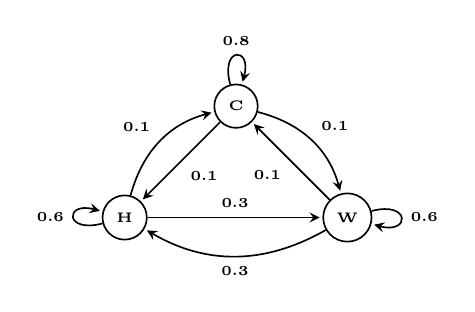
\begin{tikzpicture}[
			> = stealth, % arrow head style
			shorten > = 1pt, % don't touch arrow head to node
			auto,
			node distance = 2cm, % distance between nodes
			semithick, % line style
			font=\tiny\bfseries
			]
			
			\node[circle,draw] (qC) {C};
			\node[circle,draw] (qH) [below left of=qC] {H};
			\node[circle,draw] (qW) [below right of=qC] {W};
			
			\path[->] 	
			(qC) 	edge [loop above] node {0.8} ()
			edge [] node {0.1} (qH)
			edge [bend left] node {0.1} (qW)
			(qH) 	edge [loop left] node {0.6} ()
			edge [bend left] node {0.1} (qC)
			edge [] node {0.3} (qW)
			(qW)	edge [loop right] node {0.6} ()
			edge [bend left] node {0.3} (qH)
			edge [] node {0.1} (qC);
		\end{tikzpicture}
	\end{minipage}
	
	\begin{itemize}
		\item $\pi = [\pi_1, \pi_2, \ldots, \pi_L ]$: states' initial probability distribution $\sum_i \pi_i = 1$.
%		\item $\sum_i \pi_i = 1$.
		\item E.g. \expword{Calculate $p(H\, W\, C\, C)$ where $\pi = [\underbrace{0.1}_C, \underbrace{0.7}_H, \underbrace{0.2}_W]$}.
	\end{itemize}
	
\end{frame}

\begin{frame}
	\frametitle{\insertshortsubtitle: \insertsection}
	\framesubtitle{\insertsubsection: Hidden Markov Model}
	
	\begin{minipage}{.54\textwidth}
		\begin{itemize}
			\item $Q = \{q_1, q_2, \ldots, q_L\}$: states.
			\item $A$: transition probability matrix where $\sum_j a_{ij} = 1,\, \forall i$.
			\item $O = o_1 o_2 \ldots o_T$: sequence of observed events.
			\item $B = b_i(o_t)$: observation probabilities (\keyword{emission probabilities}), each represents the probability of generating an observation $o_t$ in a state $q_i$.
		\end{itemize}
	\end{minipage}
	\begin{minipage}{.45\textwidth}
		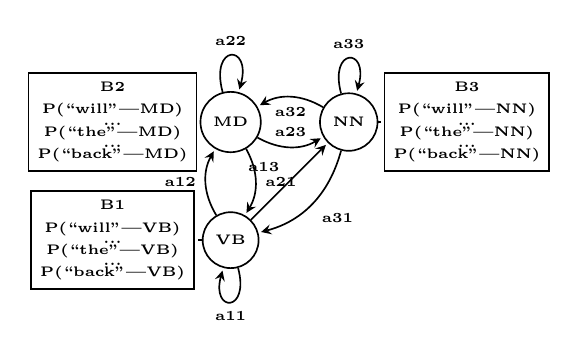
\begin{tikzpicture}[
			> = stealth, % arrow head style
			shorten > = 1pt, % don't touch arrow head to node
			auto,
			node distance = 1.5cm, % distance between nodes
			semithick, % line style
			font=\bfseries\fontsize{4}{4}\selectfont
			]
			
			\node[circle,draw] (q2) {MD};
			\node[align=center,draw] (q2e) [left of=q2] {B2\\ \\P(``will"|MD)\\...\\P(``the"|MD)\\...\\P(``back"|MD)};
			\node[circle,draw] (q3) [right of=q2] {NN};
			\node[align=center,draw] (q3e) [right of=q3] {B3\\ \\P(``will"|NN)\\...\\P(``the"|NN)\\...\\P(``back"|NN)};
			\node[circle,draw] (q1) [below of=q2] {VB};
			\node[align=center,draw] (q1e) [left of=q1] {B1\\ \\P(``will"|VB)\\...\\P(``the"|VB)\\...\\P(``back"|VB)};
			
			\path[->] 	
			(q1) 	edge [loop below] node {a11} ()
			edge [bend left] node {a12} (q2)
			edge [] node {a13} (q3)
			(q2) 	edge [loop above] node {a22} ()
			edge [bend left] node {a21} (q1)
			edge [bend right] node {a23} (q3)
			(q3)	edge [loop above] node {a33} ()
			edge [bend left] node {a31} (q1)
			edge [bend right] node {a32} (q2);
			
			\path[dashed] 	
			(q1) 	edge [] node {} (q1e)
			(q2) 	edge [] node {} (q2e)
			(q3) 	edge [] node {} (q3e);
			
		\end{tikzpicture}
	\end{minipage}
	
	\begin{itemize}
		\item $\pi = [\pi_1, \pi_2, \ldots, \pi_L ]$: states initial probability distribution.
		\item $\sum_i \pi_i = 1$.
	\end{itemize}
	
\end{frame}

\subsection{Training}

\begin{frame}
	\frametitle{\insertshortsubtitle: \insertsection}
	\framesubtitle{\insertsubsection}
	
	\begin{itemize}
		\item each tag/label $t_i$ belongs to one of the $ L $ states.
		\item Let's define \keyword{START} as sentences' start tag.
		\item \keyword{C}: Number of occurrences in the training corpus.
		\item $ M $  samples, each contains $ T $ observations, each have one tag out of $ L $ ones
	\end{itemize}
	
	\begin{block}{HMM training}
		\[
		\text{Transition probabilities: } p(t_i | t_{i-1}) = \frac{C(t_{i-1}, t_i)}{C(t_{i-1})} 
		\]\[
		\text{Emission probabilities: } p(o_i | t_i) = \frac{C(t_i, o_i)}{C(t_i)}
		\]\[
		\text{Initial distribution: } \pi_i = p(t_i | START) = \frac{C(START, t_i)}{C(START)=M}
		\]
	\end{block}
	
\end{frame}

\subsection{Estimation}

\begin{frame}
	\frametitle{\insertshortsubtitle: \insertsection}
	\framesubtitle{\insertsubsection: Labeling}
	
	\begin{itemize}
		\item Given
		\begin{itemize}
			\item a Markov model $\lambda = (A, B)$,
			\item an observations' sequence: $o = o_1 o_2 \ldots o_T$
		\end{itemize}
		\item Estimate a labels' sequence $\hat{t} = \hat{t}_1 \hat{t}_2 \ldots \hat{t}_T$
	\end{itemize}
	
	\begin{block}{Labels' decoding using HMM}
		\[
		\hat{t} = \arg\max\limits_t p(t | o) = \arg\max\limits_t \frac{p(o|t) p(t)}{p(o)} = \arg\max\limits_t p(o|t) p(t)%\text{ tel que } t = t_1 t_2 \ldots t_n
		\]
		
		\[ 
		p(o | t) \approx \prod\limits_{i=1}^T p(o_i|t_i) 
		\hskip2cm
		p(t) \approx \prod\limits_{i=1}^T p(t_i|t_{i-1}) 
		\]
		
		\[
		\hat{t} = \arg\max\limits_t \prod\limits_{i=1}^T p(o_i|t_i) p(t_i|t_{i-1})
		\]
	\end{block}
	
\end{frame}

\begin{frame}
	\frametitle{\insertshortsubtitle: \insertsection}
	\framesubtitle{\insertsubsection: Decoding (Viterbi)}
	
	\begin{block}{Viterbi}
		\scriptsize
		\begin{algorithm}[H]
			%				\vskip-1em
			\KwData{$o = o_1 \ldots o_T$, HMM $\lambda = (A, B)$ with $L$ states}
			\KwResult{$best\_path$, $prob\_path$}
			
			Create a matrix $viterbi[L, T]$\;
			
			\lForEach{state $ s = 1 \ldots L$}{
				$viterbi[s, 1] = \pi_s * p(o_1|s);\, backpointer[s, 1] = 0$
			}
			
			\ForEach{timestamp $ i = 2 \ldots T$}{
				\ForEach{state $ s = 1 \ldots L$}{
					$viterbi[s, t] = \max\limits_{s'=1}^L viterbi[s', i-1] * p(s|s') * p(o_t|s)$\;
					$backpointer[s, t] = \arg\max\limits_{s'=1}^L viterbi[s', i-1] * p(s|s') * p(o_t|s))$\;
				}
			}
			
			$prob\_path = \max\limits_{s=1}^L viterbi[s, T];\, pointer\_path = \arg\max\limits_{s=1}^L viterbi[s, T]$\;
			
			$best\_path$ is the path starting from $pointer\_path$ and following $backpointer$
			
			\Return $best\_path$, $prob\_path$\;
			
		\end{algorithm}
	\end{block}
	
\end{frame}


\section{Numerical application}

\begin{frame}
	\frametitle{\insertshortsubtitle}
	\framesubtitle{\insertsection}
	
	\begin{itemize}
		\item \textbf{Multinomial NB}: Play or not based on these categorical features: outlook (sunny, overcast, rainy), temp (hot, mild, cool), humidity (high, normal), windy (true, false)
		\item \textbf{Bernoulli NB}: Pass the exam or fail based on these boolean features: confident, studied, sick
		\item \textbf{Normal NB}: Male or female based on these numerical features: height (cm), weight (kg), footsize (cm)
		\item \textbf{HMM}: find words' grammatical categories
	\end{itemize}
	
	
\end{frame}

\subsection{Multinomial NB}

\begin{frame}
	\frametitle{\insertshortsubtitle: \insertsection}
	\framesubtitle{\insertsubsection: Example (1)}
	
	\begin{minipage}{0.35\textwidth}
		\scriptsize
		\SetTblrInner{rowsep=0pt,colsep=1pt}
		\begin{tblr}{
				colspec = {lllll},
				row{odd} = {lightblue},
				row{even} = {lightyellow},
				row{1} = {bg=darkblue, fg=white},
			} 
			%			\begin{tabular}{llllll}
				outlook & temp & humidity & windy & play \\
				sunny & hot & high & false & no \\
				sunny & hot & high & true & no \\
				overcast & hot & high & false & yes \\
				rainy & mild & high & false & yes \\
				rainy & cool & normal & false & yes \\
				rainy & cool & normal & true & no \\
				overcast & cool & normal & true & yes \\
				sunny & mild & high & false & no \\
				sunny & cool & normal & false & yes \\
				rainy & mild & normal & false & yes \\
				sunny & mild & normal & true & yes \\
				overcast & mild & high & true & yes \\
				overcast & hot & normal & false & yes \\
				rainy & mild & high & true & no \\
				%			\end{tabular}
		\end{tblr}
	\end{minipage}
	\begin{minipage}{0.64\textwidth}
		\begin{itemize}
			\item Prior probability
			\begin{itemize}
				\item $p(play=yes) = \frac{\#(play = yes)}{M} = \frac{9}{14}$
				\item $p(play=no) = \frac{\#(play = no)}{M} = \frac{5}{14}$
			\end{itemize}
			\item Likelihood probability of $ outlook=rainy $
			\begin{itemize}
				\item $p(outlook=rainy|play=yes) = \frac{\#(outlook=rainy \wedge play = yes)}{\#(play = yes)} = \frac{3}{9}$
				\item $p(outlook=rainy|play=no) = \frac{\#(outlook=rainy \wedge play = no)}{\#(play = yes)} = \frac{2}{5}$
			\end{itemize}
			\item Likelihood probability of $ temp=hot $
			\begin{itemize}
				\item $p(temp=hot|play=yes) = \frac{\#(temp=hot \wedge play = yes)}{\#(play = yes)} = \frac{2}{9}$
				\item $p(temp=hot|play=no) = \frac{\#(temp=hot \wedge play = no)}{\#(play = yes)} = \frac{2}{5}$
			\end{itemize}
		\end{itemize}
	\end{minipage}
	
\end{frame}

\begin{frame}
	\frametitle{\insertshortsubtitle: \insertsection}
	\framesubtitle{\insertsubsection: Example (2)}
	
	\begin{itemize}
		\item Likelihood probability of $ humidity=high $
		\begin{itemize}
			\item $p(humidity=high|play=yes) = \frac{\#(humidity=high \wedge play = yes)}{\#(play = yes)} = \frac{3}{9}$
			\item $p(humidity=high|play=no) = \frac{\#(humidity=high \wedge play = no)}{\#(play = yes)} = \frac{4}{5}$
		\end{itemize}
		\item Likelihood probability of $ windy=false $
		\begin{itemize}
			\item $p(windy=false|play=yes) = \frac{\#(windy=false \wedge play = yes)}{\#(play = yes)} = \frac{6}{9}$
			\item $p(windy=false|play=no) = \frac{\#(windy=false \wedge play = no)}{\#(play = yes)} = \frac{2}{5}$
		\end{itemize}
	\end{itemize}
	
	\vfill
	Given $ \vec{v} = [rainy, hot, high, false]$
	\begin{itemize}
		\item $p(play=yes|x=\vec{v}) \propto \frac{9}{14} (\frac{3}{9} \frac{2}{9} \frac{3}{9} \frac{6}{9}) = \frac{6}{567} \approx 0.0106$
		\item $p(play=no|x=\vec{v}) \propto \frac{5}{14} (\frac{2}{5} \frac{2}{5} \frac{4}{5} \frac{2}{5}) = \frac{16}{875} \approx 0.0183$
		\item $ \hat{y} = no $
	\end{itemize}
	
\end{frame}


\subsection{Bernoulli NB}

\begin{frame}
	\frametitle{\insertshortsubtitle: \insertsection}
	\framesubtitle{\insertsubsection: Example (1)}
	
	\begin{minipage}{0.5\textwidth}
		\scriptsize
		\SetTblrInner{rowsep=0pt,colsep=1pt}
		\begin{tblr}{
				colspec = {p{.2\textwidth}p{.2\textwidth}p{.2\textwidth}p{.2\textwidth}},
				row{odd} = {lightblue, font=\small},
				row{even} = {lightyellow, font=\small},
				row{1} = {darkblue, font=\bfseries},
			}
			\textcolor{white}{confident} & \textcolor{white}{studied} & \textcolor{white}{sick} & \textcolor{white}{result} \\
			1 & 0 & 0 & fail \\
			1 & 0 & 1 & pass \\
			0 & 1 & 1 & fail \\
			0 & 1 & 0 & pass \\
			1 & 1 & 1 & pass \\
		\end{tblr}
	\end{minipage}
	\begin{minipage}{0.49\textwidth}
		\begin{itemize}
			\item Prior probability
			\begin{itemize}
				\item $p(pass) = \frac{\#(pass)}{M} = \frac{3}{5}$
				\item $p(fail) = \frac{\#(fail)}{M} = \frac{2}{5}$
			\end{itemize}
		\end{itemize}
	\end{minipage}

	\begin{itemize}
		\item Prior probability
	\end{itemize}

	\begin{minipage}{0.12\textwidth}\small
		\hfill
	\end{minipage}
	\begin{minipage}{0.43\textwidth}\small
		\begin{itemize}
			\item $p(confident|pass) = \frac{2}{3}$
			\item $p(studied|pass) = \frac{2}{3}$
			\item $p(sick|pass) = \frac{2}{3}$
		\end{itemize}
	\end{minipage}
	\begin{minipage}{0.43\textwidth}\small
		\begin{itemize}
			\item $p(confident|fail) = \frac{1}{2}$
			\item $p(studied|fail) = \frac{1}{2}$
			\item $p(sick|fail) = \frac{1}{2}$
		\end{itemize}
	\end{minipage}

	\vfill
	Given $ \vec{v} = [1, 0, 0]$
	\begin{itemize}
		\item $p(pass|\vec{v}) \propto \frac{3}{5} [\frac{2}{3} (1-\frac{2}{3}) (1-\frac{2}{3})]  = \frac{2}{45} \approx 0.0444$
		\item $p(fail|\vec{v}) \propto \frac{2}{5} [\frac{1}{2} (1-\frac{1}{2}) (1-\frac{1}{2})]  = \frac{1}{20} \approx 0.05$
		\item $ \hat{y} = fail $
	\end{itemize}
	
	
\end{frame}


\subsection{Normal NB}

\begin{frame}
	\frametitle{\insertshortsubtitle: \insertsection}
	\framesubtitle{\insertsubsection: Example}
	
	\begin{minipage}{0.35\textwidth}
		\scriptsize
		\SetTblrInner{rowsep=1pt,colsep=1pt}
		\begin{tblr}{
				colspec = {llll},
				row{odd} = {lightblue, font=\small},
				row{even} = {lightyellow, font=\small},
				row{1} = {darkblue, font=\bfseries},
			}
			\textcolor{white}{height} & \textcolor{white}{weight} & \textcolor{white}{footsize} & \textcolor{white}{person} \\
			182 & 81.6 & 30 & male\\
			180 & 86.2 & 28 & male\\
			170 & 77.1 & 30 & male\\
			180 & 74.8 & 25 & male\\
			152 & 45.4 & 15 & female\\
			168 & 68.0 & 20 & female\\
			165 & 59.0 & 18 & female\\
			175 & 68.0 & 23 & female\\
		\end{tblr}
	\end{minipage}
	\begin{minipage}{0.64\textwidth}
		\begin{itemize}
			\item Prior probability: no need since the classes distribution is uniform
		\end{itemize}
		\scriptsize\SetTblrInner{rowsep=2pt,colsep=3pt}
		\begin{tblr}{
				colspec = {ccccccc},
				row{odd} = {lightblue, font=\small},
				row{even} = {lightyellow, font=\small},
				row{1,2} = {darkblue, font=\bfseries},
				cell{1}{1} = {r=2}{c},
				cell{1}{2, 4, 6} = {c=2}{c},
			}
			\textcolor{white}{person} & \textcolor{white}{height} & & \textcolor{white}{weight} & & \textcolor{white}{footsize} & \\
			& \textcolor{white}{$ \mu $} & \textcolor{white}{$ \sigma^2 $} & \textcolor{white}{$ \mu $} & \textcolor{white}{$ \sigma^2 $} &
			\textcolor{white}{$ \mu $} & \textcolor{white}{$ \sigma^2 $} \\
			male & 178 & 29.33 & 79.92 & 25.48 & 28.25 & 5.58\\
			female & 165 & 92.67 & 60.1 & 114.04 & 19 & 11.33\\
		\end{tblr}
	\end{minipage}
	
	\vfill
	Given $ \vec{v} = [183, 59, 20]$
	\begin{itemize}
		\item $ p(height=183|male) = \frac{1}{\sqrt{2\pi * 29.33}} e^\frac{-(183-165)^2}{2 * 29.33} $
		\item $ p(height=183|female) = \frac{1}{\sqrt{2\pi * 92.67}} e^\frac{-(183-165)^2}{2 * 92.67} $
	\end{itemize}
	
	
\end{frame}

\subsection{HMM}

\begin{frame}
	\frametitle{\insertshortsubtitle: \insertsection}
	\framesubtitle{\insertsubsection: Example}
	
	\begin{exampleblock}{Example of a training corpus}
		\hspace{12pt}
		\begin{minipage}{0.38\textwidth}
			\begin{enumerate}
				\item a/\textsubscript{D} fish/\textsubscript{N} can/\textsubscript{V} swim/\textsubscript{V}
				\item I/\textsubscript{P} want/\textsubscript{V} the/\textsubscript{D} can/\textsubscript{N}
%				\item fish/\textsubscript{N} eat/\textsubscript{V} fish/\textsubscript{N}
%				\item you/\textsubscript{P} fish/\textsubscript{v}
			\end{enumerate}
		\end{minipage}
		\begin{minipage}{0.15\textwidth}
			\hfill
		\end{minipage}
		\begin{minipage}{0.38\textwidth}
			\begin{enumerate}\addtocounter{enumi}{2}
%				\item a/\textsubscript{D} fish/\textsubscript{N} can/\textsubscript{V} swim/\textsubscript{V}
%				\item I/\textsubscript{P} want/\textsubscript{V} the/\textsubscript{D} fish/\textsubscript{N}
				\item fish/\textsubscript{N} eat/\textsubscript{V} fish/\textsubscript{N}
				\item you/\textsubscript{P} fish/\textsubscript{V} 
				\item fish/\textsubscript{V} the/\textsubscript{D} fish/\textsubscript{N}
			\end{enumerate}
		\end{minipage}
	\end{exampleblock}

	\begin{itemize}
		\item the set of available tags is \{D, N, V, P\} (in our case: states)
		\item $ M = 5 $ the number of training samples
		\item each word is an observation
		\item In this case, the set of available observations is \{a, fish, can, swim, I, want, the, eat, you\}
	\end{itemize}
	
\end{frame}

\begin{frame}
	\frametitle{\insertshortsubtitle: \insertsection}
	\framesubtitle{\insertsubsection: Probability calculation}
	
	\begin{itemize}
		\item Let us calculate \textbf{p(I/\textsubscript{P} can/\textsubscript{V} fish/\textsubscript{N})}
		\item which is equivalent to \textbf{p( P V N \textbar\ I can fish )}
		\item Emission probabilities
		\begin{itemize}
			\item $ p(I|P) = \frac{\#(I,P)}{\#P} = \frac{1}{2} $ \hspace{6pt} 
			$ p(can|V) = \frac{\#(can,V)}{\#V} = \frac{1}{6} $ \hspace{6pt}
			$ p(fish|N) = \frac{\#(fish,N)}{\#N} = \frac{4}{5} $
			\item $ p(I\ can\ fish | P\ V\ N) = p(I|P)\ p(can|V)\ p(fish|N) = \frac{1}{2} \frac{1}{6} \frac{4}{5} = \frac{1}{15}$
		\end{itemize}
		\item Transition probabilities
		\begin{itemize}
			\item $ \pi_P = \frac{\#(START\ P)}{M} = \frac{2}{5} $ \hspace{6pt} 
			$ p(V|P) = \frac{\#(P\ V)}{\#P} = \frac{2}{2} $ \hspace{6pt} 
			$ p(N|V) = \frac{\#(V\ N)}{\#V} = \frac{1}{6} $
			\item $ p(P\ V\ N) = \pi_P\ p(V|P)\ p(N|V) = \frac{2}{5} \frac{2}{2} \frac{1}{6} = \frac{1}{15}$
		\end{itemize}
		\item Final probability
		\begin{itemize}
			\item $ p(P\ V\ N | I\ can\ fish) \propto p(I\ can\ fish | P\ V\ N)\ p(P\ V\ N) = \frac{1}{15} \frac{1}{15} = \frac{1}{225}$
		\end{itemize}
	\end{itemize}

%	$ p(I|P) = \frac{\#(I,P)}{\#D} = \frac{1}{2} $
%	
%	$ p(can|V) = \frac{\#(can,V)}{\#V} = \frac{1}{5} $
%	
%	$ p(fish|N) = \frac{\#(fish,N)}{\#N} = \frac{3}{4} $
%	
%	$ \pi_P = \frac{\#(START\ P)}{M} = \frac{2}{4} $
%	
%	$ p(V|P) = \frac{\#(P\ V)}{\#P} = \frac{2}{2} $
%	
%	$ p(N|V) = \frac{\#(V\ N)}{\#V} = \frac{1}{5} $
	
	
\end{frame}

\begin{frame}
	\frametitle{\insertshortsubtitle: \insertsection}
	\framesubtitle{\insertsubsection: Training (All the model)}
	
	\begin{itemize}
		\item the value is: \textbf{p(column \textbar\ row)}
	\end{itemize}
	\vfill

	\centering
	
	\SetTblrInner{rowsep=1pt,colsep=3pt}
	\begin{tblr}{
			colspec = {cccccccccccccccc},
%			hlines = {1pt, black},
			cell{1}{3} = {c=4}{c},
			cell{1}{8} = {c=9}{c},
			cell{even}{1} = {darkred, font=\bfseries, fg=white},
			cell{odd}{1} = {darkgreen, font=\bfseries, fg=white},
			cell{even}{3-6} = {lightred},
			cell{odd}{3-6} = {lightgreen},
			cell{even}{8-16} = {lightred},
			cell{odd}{8-16} = {lightgreen},
			cell{1}{3,8} = {darkblue, font=\bfseries, fg=white},
			cell{2}{3-6,8-16} = {blue, font=\bfseries, fg=yellow},
			cell{1,2}{1} = {white},
			cell{7}{8-16} = {white},
		}
		  &\hspace{6pt}& Transition &  &  &  & \hspace{6pt} & Emission &  &  &  &  &  &  & &  \\
		  && D & N & V & P & & a & fish & can & swim & I & want & the & eat & you \\
		D && $ 0 $ & $ 1 $ & $ 0 $ & $ 0 $ && $ \frac{1}{3} $ & $0$ & $0$ & $0$ & $0$ & $0$ & $\frac{2}{3}$ & $0$ & $0$ \\
		N && $ 0 $ & $ 0 $ & $ \frac{2}{5} $ & $ 0 $ && $0$ & $\frac{4}{5}$ & $\frac{1}{5}$ & $0$ & $0$ & $0$ & $0$ & $0$ & $0$ \\
		V && $ \frac{1}{3} $ & $ \frac{1}{6} $ & $ \frac{1}{6} $ & $ 0 $ & & $0$ & $\frac{1}{3}$ & $\frac{1}{6}$ & $\frac{1}{6}$ & $0$ & $\frac{1}{6}$ & $0$ & $\frac{1}{6}$ & $0$ \\
		P && $ 0 $ & $ 0 $ & $ 1 $ & $ 0 $ && $0$ & $0$ & $0$ & $0$ & $\frac{1}{2}$ & $0$ & $0$ & $0$ & $\frac{1}{2}$ \\
		$ \pi $ && $ \frac{1}{5} $ & $ \frac{1}{5} $ & $ \frac{1}{5} $ & $ \frac{2}{5} $ &&  &  &  &  &  &  &  &  &  \\
	\end{tblr}

	%		  & D & N & V & P & 
	%		  & $ 0 $ & $ 1 $ & $ 0 $ & $ 0 $ &
	%		  & $ 0 $ & $ 0 $ & $ \frac{2}{5} $ & $ 0 $ &
	%		  & $ \frac{1}{3} $ & $ \frac{1}{6} $ & $ \frac{1}{6} $ & $ 0 $ & 
	%		  & $ 0 $ & $ 0 $ & $ 1 $ & $ 0 $ &
	
\end{frame}

\begin{frame}
	\frametitle{\insertshortsubtitle: \insertsection}
	\framesubtitle{\insertsubsection: Tags decoding using Viterbi}
	
	
	\tiny\SetTblrInner{rowsep=1pt,colsep=3pt}
	\begin{tblr}{
			colspec = {lllll},
%			row{odd} = {lightblue, font=\small},
%			row{even} = {lightyellow, font=\small},
			row{1} = {darkblue, font=\bfseries},
			column{1} = {darkblue, font=\bfseries},
			cell{2, 6, 10, 14}{1,2} = {r=4}{l},
			hline{2-18} = {1pt,solid},
			cell{1}{1} = {white},
			cell{4,8,11,15}{3} = {yellow},
			cell{4,12,15}{5} = {yellow},
			cell{8}{5} = {orange},
		}
		 & \textcolor{white}{fish} & \textcolor{white}{can} && \textcolor{white}{fish} \\
		\textcolor{white}{D} & $\scriptstyle \pi_D * p(fish|D) $ \linebreak= $\scriptstyle \frac{1}{5} * 0 = 0 $ 
		   & $\scriptstyle viterbi[D,1] * p(D|D) * p(can|D) = 0 * 0 * 0 = 0$  && $\scriptstyle viterbi[D,2] * p(D|D) * p(fish|D) = 0 * 0 * 0 = 0 $\\
		&  & $\scriptstyle viterbi[N,1] * p(D|N) * p(can|D) = \frac{4}{25} * 0 * 0 = 0$  && $\scriptstyle viterbi[N,2] * p(D|N) * p(fish|D) = \frac{1}{750} * 0 * 0 = 0$\\
		&  & $\scriptstyle viterbi[V,1] * p(D|V) * p(can|D) = \frac{1}{25} * \frac{1}{3} * 0 = 0 $  && $\scriptstyle viterbi[V,2] * p(D|V) * p(fish|D) = \frac{4}{375} * \frac{1}{3} * 0 = 0$\\
		&  & $\scriptstyle viterbi[P,1] * p(D|P) * p(can|D) = 0 * 0 * 0 = 0$  && $\scriptstyle viterbi[P,2] * p(D|P) * p(fish|D) = 0 * 0 * 0 = 0$\\
		
		\textcolor{white}{N} & $\scriptstyle \pi_N * p(fish|N) $ \linebreak= $\scriptstyle \frac{1}{5} * \frac{4}{5} = \frac{4}{25} $  
		   & $\scriptstyle viterbi[D,1] * p(N|D) * p(can|N) = 0 * 0 * \frac{1}{5} = 0 $  && $\scriptstyle viterbi[D,2] * p(N|D) * p(fish|N) = 0 * 1 * \frac{4}{5} = 0 $\\
		&  & $\scriptstyle viterbi[N,1] * p(N|N) * p(can|N) = \frac{4}{25} * 0 * \frac{1}{5} = 0 $  && $\scriptstyle viterbi[N,2] * p(N|N) * p(fish|N) = \frac{1}{750} * 0 * \frac{4}{5} = 0 $\\
		&  & $\scriptstyle viterbi[V,1] * p(N|V) * p(can|N) = \frac{1}{25} * \frac{1}{6} * \frac{1}{5} = \frac{1}{750} $  && $\scriptstyle viterbi[V,2] * p(N|V) * p(fish|N) = \frac{4}{375} * \frac{1}{6} * \frac{4}{5} = \frac{8}{5625} $\\
		&  & $\scriptstyle viterbi[P,1] * p(N|P) * p(can|N) = 0 * 0 * \frac{1}{5} = 0$  && $\scriptstyle viterbi[P,2] * p(N|P) * p(fish|N) = 0 * 0 * \frac{4}{5} = 0 $\\
		
		\textcolor{white}{V} & $\scriptstyle \pi_V * p(fish|V) $ \linebreak= $\scriptstyle \frac{1}{5} * \frac{1}{5} = \frac{1}{25} $ 
		   & $\scriptstyle viterbi[D,1] * p(V|D) * p(can|V) = 0 * 0 * \frac{1}{6} = 0$  && $\scriptstyle viterbi[D,2] * p(V|D) * p(fish|V) = 0 * 0 * \frac{1}{3} = 0 $\\
		&  & $\scriptstyle viterbi[N,1] * p(V|N) * p(can|V) = \frac{4}{25} * \frac{2}{5} * \frac{1}{6} = \frac{4}{375} $  && $\scriptstyle viterbi[N,2] * p(V|N) * p(fish|V) = \frac{1}{750} * \frac{2}{5} * \frac{1}{3} = \frac{1}{5625}$\\
		&  & $\scriptstyle viterbi[V,1] * p(V|V) * p(can|V) = \frac{1}{25} * \frac{1}{6} * \frac{1}{6} = \frac{1}{900}$  && $\scriptstyle viterbi[V,2] * p(V|V) * p(fish|V) = \frac{4}{375} * \frac{1}{6} * \frac{1}{3} = \frac{2}{3375}$\\
		&  & $\scriptstyle viterbi[P,1] * p(V|P) * p(can|V) = 0 * 1 * \frac{1}{6} = 0$  && $\scriptstyle viterbi[P,2] * p(V|P) * p(fish|V) = 0 * 1 * \frac{1}{3} = 0 $\\
		
		\textcolor{white}{P} & $\scriptstyle \pi_P * p(fish|P) $ \linebreak= $\scriptstyle \frac{2}{5} * 0 = 0 $ 
		   & $\scriptstyle viterbi[D,1] * p(P|D) * p(can|P) = 0 * 0 * 0 = 0$  && $\scriptstyle viterbi[D,2] * p(P|D) * p(fish|P) = 0 * 0 * 0 = 0 $\\
		&  & $\scriptstyle viterbi[N,1] * p(P|N) * p(can|P) = \frac{4}{25} * 0 * 0 = 0 $  && $\scriptstyle viterbi[N,2] * p(P|N) * p(fish|P) = \frac{4}{375} * 0 * 0 = 0$\\
		&  & $\scriptstyle viterbi[V,1] * p(P|V) * p(can|P) = \frac{1}{25} * 0 * 0 = 0 $  && $\scriptstyle viterbi[V,2] * p(P|V) * p(fish|P) = \frac{4}{375} * 0 * 0 = 0$\\
		&  & $\scriptstyle viterbi[P,1] * p(P|P) * p(can|P) = 0 * 0 * 0 = 0$  && $\scriptstyle viterbi[P,2] * p(P|P) * p(fish|P) = 0 * 0 * 0 = 0 $\\

	\end{tblr}
	
\end{frame}

%\insertbibliography{ML-RN}{*}

\end{document}

